\documentclass{tufte-handout}

\title{Session 14}

\author[Pepe García]{Pepe García}

%\date{28 March 2010} % without \date command, current date is supplied

%\geometry{showframe} % display margins for debugging page layout

\usepackage{graphicx} % allow embedded images
  \setkeys{Gin}{width=\linewidth,totalheight=\textheight,keepaspectratio}
  \graphicspath{{../img/}} % set of paths to search for images
\usepackage{listings}  % for code
\usepackage{amsmath}  % extended mathematics
\usepackage{booktabs} % book-quality tables
\usepackage{units}    % non-stacked fractions and better unit spacing
\usepackage{multicol} % multiple column layout facilities
\usepackage{lipsum}   % filler text
\usepackage{fancyvrb} % extended verbatim environments
  \fvset{fontsize=\normalsize}% default font size for fancy-verbatim environments
\usepackage{xcolor}   % for colors

\definecolor{codegreen}{rgb}{0,0.6,0}
\definecolor{codegray}{rgb}{0.5,0.5,0.5}
\definecolor{codepurple}{rgb}{0.58,0,0.82}
\definecolor{backcolour}{rgb}{1,1,1}

\lstdefinestyle{mystyle}{
    backgroundcolor=\color{backcolour},
    commentstyle=\color{codegreen},
    keywordstyle=\color{magenta},
    numberstyle=\tiny\color{codegray},
    stringstyle=\color{codepurple},
    basicstyle=\ttfamily\footnotesize,
    breakatwhitespace=false,
    breaklines=true,
    captionpos=b,
    keepspaces=true,
    numbersep=5pt,
    showspaces=false,
    showstringspaces=false,
    showtabs=false,
    tabsize=4
}

\lstset{style=mystyle}

% Standardize command font styles and environments
\newcommand{\doccmd}[1]{\texttt{\textbackslash#1}}% command name -- adds backslash automatically
\newcommand{\docopt}[1]{\ensuremath{\langle}\textrm{\textit{#1}}\ensuremath{\rangle}}% optional command argument
\newcommand{\docarg}[1]{\textrm{\textit{#1}}}% (required) command argument
\newcommand{\docenv}[1]{\textsf{#1}}% environment name
\newcommand{\docpkg}[1]{\texttt{#1}}% package name
\newcommand{\doccls}[1]{\texttt{#1}}% document class name
\newcommand{\docclsopt}[1]{\texttt{#1}}% document class option name
\newenvironment{docspec}{\begin{quote}\noindent}{\end{quote}}% command specification environment

\begin{document}

\maketitle% this prints the handout title, author, and date

\begin{abstract}
  \noindent
  In this async session you'll go over a series of exercises to learn how to
  model data depending on the problem at hand.
\end{abstract}

%\printclassoptions

\section{DNS}\label{sec:dns}

In this first example we'll try to model what a DNS server does.

\begin{marginfigure}%
  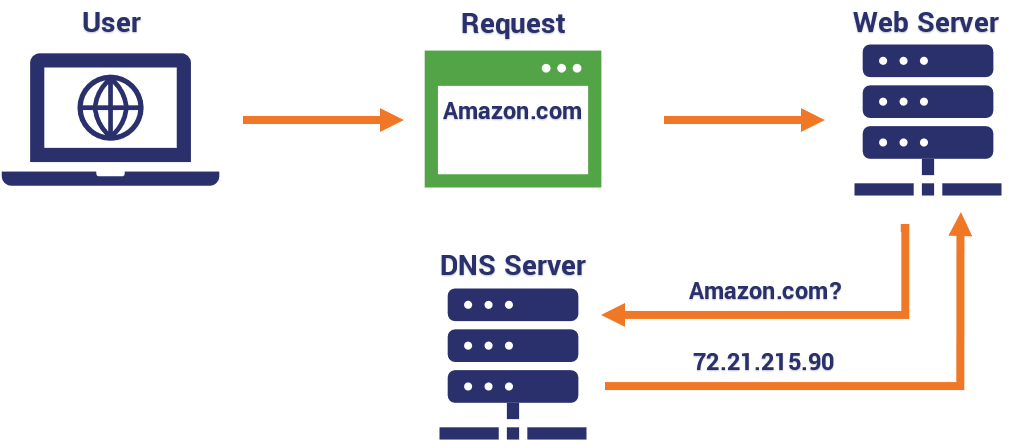
\includegraphics[width=\linewidth]{dns.png}
  \caption{\newthought{the Domain Name System} is the subsystem of the Internet in charge of
    translating from domain names to IP addresses.  Each computer connected to the
    Internet has an IP address associated so that other computers can refer to it.
    These addresses look like \textbf{102.43.250.21}, making it fairly hard to
    remember them all.\\Luckily, \textbf{DNS} allows us to map domain names, such as
    \textbf{google.com} to IP addresses like \textbf{102.43.250.21}}
  \label{fig:marginfig}
\end{marginfigure}



\subsection{Calling functions}\label{sec:callingfunctions}

The syntax for calling functions is the following:

\begin{lstlisting}[language=Python]
function_name(parameter1, parameter2, parameterN)
\end{lstlisting}

When naming functions we will need to apply the same naming rules as
for variables.

We have already seen some functions, such as \textbf{print()},
\textbf{type()}, \textbf{str()}, etc.  We used them as follows:

\begin{lstlisting}[language=Python]
type('hello')
str(3)
int(True)
\end{lstlisting}

Notice that so far, we have used all these functions by passing only
one argument, but there are others that can receive more than one
argument.

\begin{lstlisting}[language=Python]
def area_square(side):
    return side * side
\end{lstlisting}

\pagebreak

\bibliography{session14}
\bibliographystyle{plainnat}

\end{document}
